\subsection{closest\_point}
Ahora implementar la función closest\_point, siguiendo las recomendaciones dadas por el docente:

\begin{lstlisting}[language=C++,
                   directivestyle={\color{black}}
                   emph={int,char,double,float,unsigned},
                   emphstyle={\color{blue}}
                  ]
function masCercano(puntoConsulta, p1, p2) {
  if (!p1) {
    return p2;
  }
  if (!p2) {
    return p1;
  }
  return (distanceSquared(puntoConsulta, p1) < distanceSquared(puntoConsulta, p2))? p1 : p2;
}

function closestPoint(node, point, depth = 0, best = null) {
  if (!node) {
    return null;
  }
  var subTree1 = node.left;
  var subTree2 = node.right;
  if (point[depth%k] >= node.point[depth%k]) {
    subTree1 = node.right;
    subTree2 = node.left;
  }
  best = masCercano(point, closestPoint(subTree1, point, depth + 1), node.point);
  if (distanceSquared(point, best) > Math.abs(point[depth%k] - node.point[depth%k])) {
    best = masCercano(point, closestPoint(subTree2, point, depth + 1), node.point);
  }
  return best;
}
\end{lstlisting}

\begin{figure}[H]
 \centering
 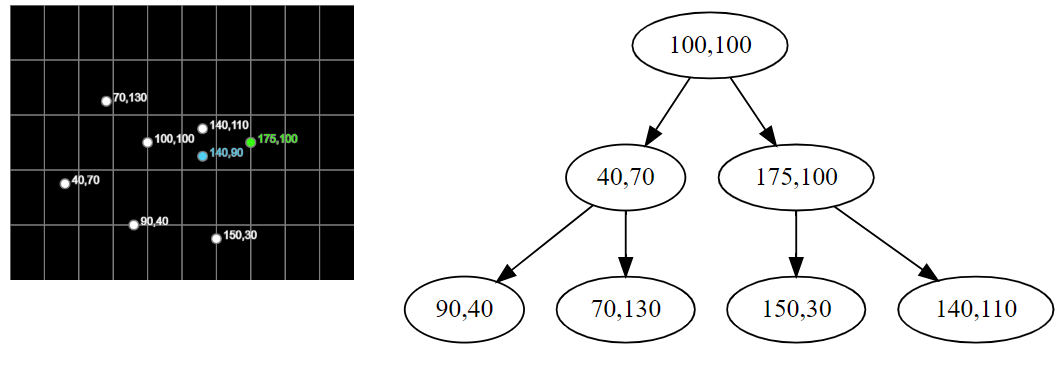
\includegraphics[width=1\textwidth]{images/closestPoint.PNG}
 \label{fig:act-7-closestPoint}
\end{figure}
Podemos apreciar el punto mas cercano de color \textcolor{green}{verde} el cual es [160,100].